\documentclass[a4paper,10pt]{article}
\usepackage[top=0.5in, bottom=1in, left=1in, right=1in]{geometry}
\usepackage[utf8]{inputenc}
\usepackage{mathptmx}  % Times New Roman font style
\usepackage{setspace}
\usepackage{titlesec}
\usepackage{hyperref}
\usepackage{graphicx} % For including images
\usepackage{xcolor}

\onehalfspacing  % Set line spacing to 1.5

% Customize section titles
\titleformat{\section}{\normalsize\bfseries}{\thesection.}{1em}{}
\titleformat{\subsection}{\normalsize\bfseries}{\thesubsection.}{1em}{}
\titleformat{\subsubsection}{\normalsize\itshape}{\thesubsubsection.}{1em}{}

% Redefine \maketitle to adjust title and author formatting
\makeatletter
\renewcommand{\maketitle}{
  \begin{center}
    {\fontsize{12pt}{14pt}\selectfont\bfseries\@title\par}
    \vskip 1em
    {\normalsize\@author\par}
    \vskip 1em
  \end{center}
}
\makeatother

\title{Self-Adaptive Systems: Methodologies for Reusability and Security}
\author{Mutasem Salloum (ms227fm) \\ Rashed Qazizada (rq222ah)}
\date{}

\begin{document}

\maketitle

\begin{abstract}
This report investigates two core research questions: (1) What are the current methodologies and approaches for achieving reusability and security in self-adaptive software systems (SAS)? and (2) What are the benefits and challenges of implementing secure and reusable components in these systems? The study examines frameworks such as Autonomic Software Product Line Engineering (ASPLe) and code-level adaptation methods, which support modularity, flexibility, and adaptability. Key findings indicate that reusability significantly reduces development costs and enhances resilience but requires integrated security measures to mitigate risks in critical environments. This research highlights the importance of combining systematic reuse strategies with security-focused metrics to build adaptable and secure SAS. Future directions include automating component evaluation processes and tailoring reuse methodologies to domain-specific needs.
\end{abstract}

\section{Introduction}

As modern software systems grow in complexity, there is a rising demand for systems that can adapt autonomously to dynamic conditions. Self-adaptive systems (SAS) are designed to meet this need, allowing software to monitor, analyse, and adjust its behaviour based on environmental changes without human intervention. In critical areas such as healthcare, cloud computing, and autonomous vehicles, this capability is essential to maintain continuous functionality despite shifting requirements or unexpected conditions. Achieving this adaptability efficiently requires the reuse of modular components that can be applied across various contexts, reducing both development time and costs.

This report investigates two research questions central to the advancement of SAS:

\begin{itemize}
  
    \item \textbf{RQ1:} What are the current methodologies and approaches used to achieve reusability and security in self-adaptive software systems?
        \item \textbf{RQ2:} What are the benefits and challenges of implementing secure and reusable components in self-adaptive software systems?
\end{itemize}

To address these questions, we need to understand a few concepts:

\begin{itemize}
    \item \textbf{Self-Adaptive Software System (SASS):} A system that can modify its behaviour and structure in response to changes in its environment, its own internal state, or its goals.
    
    \item \textbf{ASPLe (Autonomic Software Product Line Engineering):} ASPLe organizes SAS development into domain engineering, specialization, and integration stages, promoting systematic reuse of components across different applications. This modular approach saves time and supports consistent quality by allowing components to be adapted with minimal effort.
    
    \item \textbf{Code-level adaptation methods:} This strategy focuses on reusability at the coding level, allowing adaptation within specific modules. Code-level adaptation enables flexibility on a smaller scale, complementing the higher-level reusability of frameworks like ASPLe, though it may encounter scalability challenges in larger systems.
    
\end{itemize}

The motivation behind these research questions originates from the need to balance adaptability and security in SAS. While reusability can enhance efficiency and resilience, the absence of integrated security measures in reusable components can create potential vulnerabilities, particularly in critical environments. This study investigates the methodologies for reusability and the essential role of security in the development and application of self-adaptive software systems. This report provides insights into these challenges and suggests future directions for enhancing SAS with more secure and flexible reusable components, offering a foundation for further research on building robust adaptive systems that can evolve with changing conditions.
\section{Approach or Method}

To explore and answer the research questions, we conducted a literature review focusing on recent studies related to self-adaptive systems (SAS), particularly those emphasizing modularity, reuse, and adaptive security. In alignment with the project’s requirements, all articles were selected from Norwegian List Level 2 journals, ensuring a high standard of peer-reviewed quality and relevance in the field.

\subsection{Literature Review}

The literature review involved exploring academic databases, including IEEE Xplore, ScienceDirect, and SpringerLink, using search terms such as “self-adaptive systems,” “reuse,” “security,” and related terms. Articles were selected based on their relevance to the research questions and publication date (2020–2024). The review aimed to highlight methodologies, challenges, and opportunities in achieving reusability and security within self-adaptive systems.

\begin{enumerate}
    \item \textbf{ASPLe:} A methodology for reuse in self-adaptive systems, detailing a structured approach for developing reusable components \cite{Nadeem2020}.
    
    \item \textbf{Security and safety in SAS:} This article discusses security challenges in adaptive systems, especially in high-risk environments \cite{Pekaric2023}.
    
    \item \textbf{Code-level adaptation for SAS:} This study examines code-level techniques to enhance flexibility and adaptability within SAS, complementing broader reuse strategies \cite{Korra2022}.
\end{enumerate}

\subsection{Analyzing Methodologies}

Each methodology was analyzed for its contributions to modularity, adaptability, and security:

\begin{itemize}
    \item \textbf{ASPLe (Autonomic Software Product Line Engineering):} This methodology divides SAS development into domain engineering, specialization, and integration stages, creating modular artifacts for reuse. This approach supports consistent quality and adaptability across different SAS applications \cite{Nadeem2020}.
    
    \item \textbf{Code-Level Adaptation Techniques:} These techniques focus on adaptable coding practices to enable flexibility at a more granular level. Code-level adaptation is particularly beneficial for implementing fine-grained adjustments within specific modules, complementing the broader reuse strategy provided by frameworks like ASPLe \cite{Korra2022}.
\end{itemize}

This literature review provides a foundational understanding of the methodologies, challenges, and practices critical to addressing the research questions on reusability and security in SAS.


\section{Results}

This section presents the findings related to the research questions on reusable methodologies in self-adaptive systems (SAS). The results highlight the ASPLe methodology, a proposed algorithm for adaptive component development, and component metrics for evaluation, emphasizing original insights derived from the analysis.

\subsection{ASPLe Methodology}

The \textbf{Autonomic Software Product Line Engineering (ASPLe)} methodology provides process support for systematic reuse in self-adaptive systems. It is built on the \textbf{Autonomic Software Product Lines (ASPL)} strategy, addressing key challenges in modularity, reuse, and variability. ASPLe divides SAS development into three primary stages: \textit{Domain Engineering}, \textit{Specialization}, and \textit{Integration}, enabling systematic reuse of modular components across diverse domains \cite{Nadeem2020}.

\begin{figure}[ht]
\centering
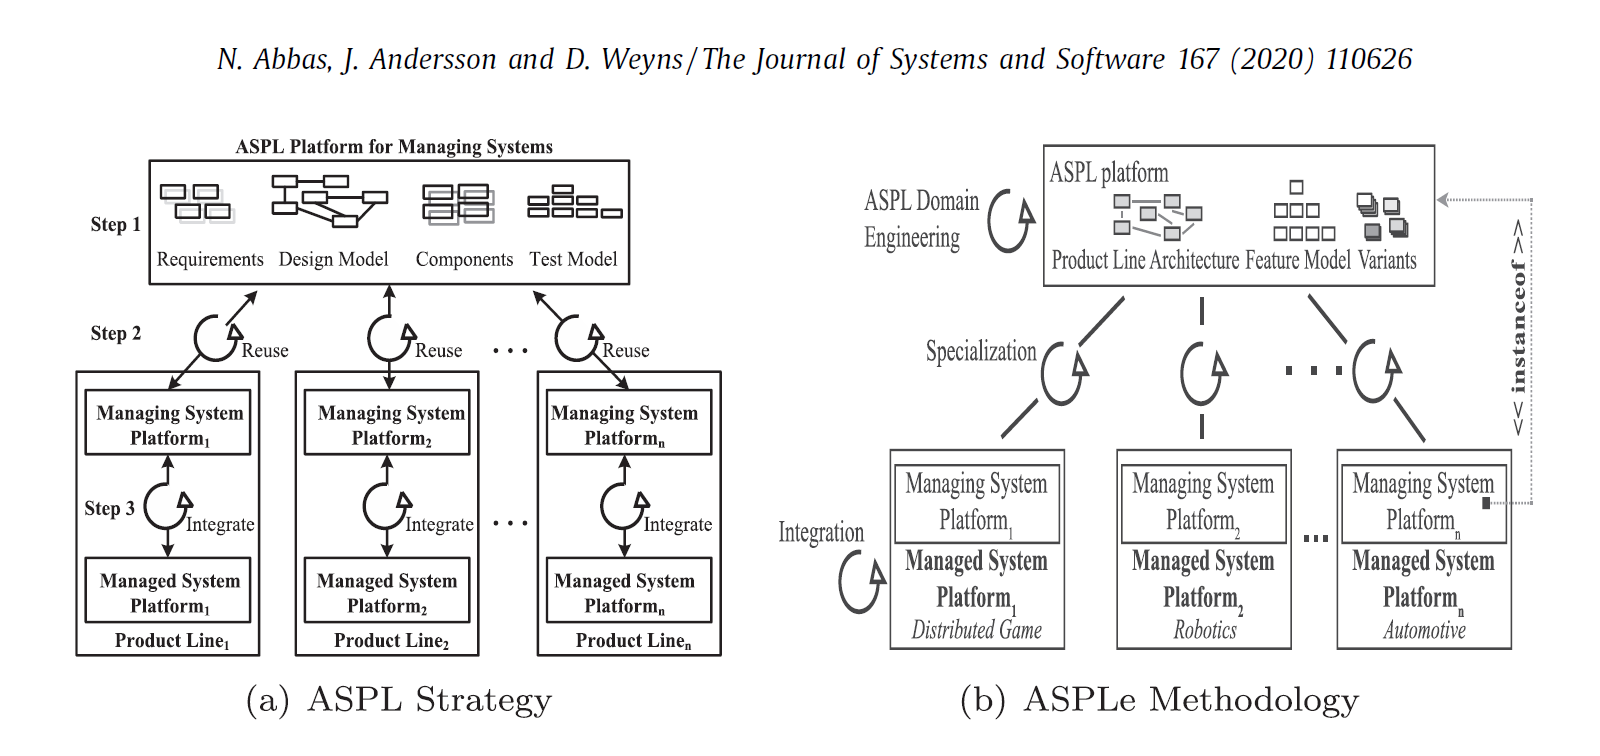
\includegraphics[width=0.8\textwidth]{asple_diagram.png}
\caption{ASPLe Methodology Overview}
\label{fig:asple}
\end{figure}

A core element of ASPLe is the \textbf{Extended Architectural Reasoning Framework (eARF)}, which guides designers in mapping self-adaptation requirements to architectural tactics using domain Quality Attribute Scenarios (dQAS). This process ensures that reusable components address adaptability, scalability, and security requirements effectively. 

\textbf{Benefits and Challenges:} ASPLe reduces complexity, promotes systematic reuse, and enhances flexibility in design. However, integrating domain-specific customizations and managing platform compatibility can introduce challenges, requiring detailed process support.

\subsection{Proposed Algorithm for Adaptive Component Development}

The proposed algorithm provides a systematic approach to developing reusable components for SAS. This algorithm focuses on deriving new insights by identifying, adapting, and testing reusable components in dynamic environments. The stages include:

\begin{enumerate}
    \item \textbf{Component Identification}: Identify potential reusable modules based on system requirements and functionality.
    \item \textbf{Metric Evaluation}: Evaluate components using specific metrics to ensure suitability for reuse. Metrics include:
        \begin{itemize}
            \item \textbf{Component Efficiency Metrics (CEM)}: Measures execution time and resource usage.
            \item \textbf{Component Semantic Efficiency Measurement (CSEM)}: Assesses code maintainability and readability.
            \item \textbf{Component Reliability Metrics (CRM)}: Evaluates defect-free operation probability over time.
            \item \textbf{Component Functional Metrics (CFM)}: Checks functionality, precision, and interoperability.
            \item \textbf{Component Customer Satisfaction Measurement (CCSM)}: Gauges satisfaction based on user feedback.
            \item \textbf{Component Cost Metrics (CCM)}: Analyzes development and integration costs.
        \end{itemize}
    \item \textbf{Component Adaptation}: Modify components to meet adaptability criteria, ensuring compatibility across contexts.
    \item \textbf{Repository Management}: Store components with metadata in a centralized repository for efficient retrieval.
    \item \textbf{Integration and Testing}: Integrate components into new projects and conduct rigorous testing.
\end{enumerate}

\textbf{Benefits and Challenges:} This algorithm fosters component reusability, reducing development time and costs. However, challenges include dependency management, adaptation complexity, and integration testing overhead, particularly in large-scale or legacy systems.

\subsection{Deriving Original Insights}

Through analysis of ASPLe and the proposed algorithm, this study identifies the following insights:
\begin{itemize}
    \item \textbf{Criticality of Metrics} Incorporating detailed metrics ensures components meet adaptability and reliability criteria, reducing risks in SAS deployment.
    \item \textbf{Integration Challenges} Seamless integration of reusable components requires advanced dependency management and robust testing frameworks.
    \item \textbf{Security in Reuse} Security measures must be embedded during component development, not as an afterthought, to address vulnerabilities.
\end{itemize}

These insights pave the way for developing more secure and adaptable SAS, addressing gaps in existing methodologies and advancing practical implementation strategies.

\subsection{Summary of Findings}

The results demonstrate that systematic reuse methodologies, when combined with robust evaluation and integration processes, can significantly improve adaptability and security in SAS. By leveraging ASPLe and adaptive component development algorithms, SAS can meet dynamic system requirements while maintaining high standards of quality and resilience.




% End of Results section
\section{Discussion}

The findings underscore the practical benefits and challenges associated with implementing reusable components in self-adaptive systems (SAS). This discussion interprets the results, reflects on their implications, and suggests areas for future research.

\subsection{Interpretation of Results}

The ASPL strategy, ASPLe methodology, and the proposed algorithm provide a comprehensive view of current methodologies for achieving reusability in SAS. However, the lack of integrated security highlights a significant challenge that must be addressed to ensure the safe deployment of SAS in sensitive environments.

Our analysis highlights the \textbf{critical role of metrics} in component evaluation. Metrics such as CEM and CRM are indispensable for ensuring adaptability, reliability, and scalability. Furthermore, embedding security measures during component evaluation—not as an afterthought—is essential to mitigate potential vulnerabilities in adaptive systems. This insight extends prior work by emphasizing security integration as a primary consideration during reuse, which has been underexplored in existing methodologies.

\subsection{Implications for Practice}

Implementing these methodologies and algorithms can lead to more efficient software development processes, particularly in domains where adaptability and reliability are critical. Organizations can benefit from reduced development time and costs by reusing well-tested components and combining real-time responsiveness with ASPLe’s systematic reuse and the proposed algorithm’s code-level adaptability.

To address identified challenges, organizations should consider adopting:
\begin{itemize}
    \item \textbf{Dependency Management Frameworks:} Tools that automate the resolution of component dependencies to streamline integration and testing.
    \item \textbf{Real-Time Metric Evaluation Tools:} Systems that enable dynamic assessment of components, ensuring reliability and adaptability in changing conditions.
    \item \textbf{Integrated Security Protocols:} Processes to embed security considerations during the design, evaluation, and adaptation of components.
\end{itemize}
\subsection{Comparison with Existing Literature}

Our findings confirm the importance of modularity and reuse in software engineering, as highlighted in prior research. The ASPLe methodology advances traditional software product line engineering by introducing self-adaptive properties, effectively addressing a gap noted in earlier studies \cite{Nadeem2020}. Additionally, the proposed algorithm enhances this by focusing on code-level adaptations, providing a detailed, practical approach that complements higher-level reuse strategies. 

This study distinguishes itself by emphasizing the critical need to integrate security into reuse practices, a consideration often neglected in existing frameworks. By addressing this gap, the research offers new perspectives on how adaptability and security can be balanced effectively in the development of SAS.

\subsection{Limitations and Future Work}

Despite the benefits, several limitations exist. First, evaluating components using multiple metrics can be time-intensive, potentially slowing down the development process. Second, dependency issues during component integration can lead to unforeseen challenges, particularly in large-scale or legacy systems.

Future research should focus on developing \textbf{automated tools} to streamline the evaluation process and reduce the time required. Customizing metrics for specific domains would enhance their relevance and effectiveness, while improved documentation and training could mitigate integration issues. Additionally, integrating security metrics directly into reuse methodologies can address vulnerabilities more effectively.

\textbf{Proposed Research Directions:}
\begin{itemize}
    \item Development of domain-specific metrics for adaptive systems.
    \item Automation of component evaluation and dependency resolution.
    \item Incorporation of security-focused protocols in adaptive frameworks.
\end{itemize}

% End of Discussion section
\section{Conclusion}

This study investigated methodologies for achieving reusability and security in self-adaptive systems (SAS), focusing on the ASPL strategy, ASPLe methodology, and a proposed algorithm for adaptive component development. The findings highlight that reusability significantly reduces development time and costs while enhancing adaptability and scalability. Metrics such as CEM and CRM play a critical role in evaluating component suitability, and embedding security measures during reuse is essential for mitigating vulnerabilities in sensitive applications.

Despite these benefits, challenges such as dependency management, adaptation complexity, and the lack of integrated security measures require further attention. Future research should focus on automating component evaluation, integrating security-focused metrics, and tailoring reuse methodologies to domain-specific needs. Addressing these challenges will enable the development of more adaptable, secure, and efficient SAS capable of meeting evolving demands across industries.


% End of Conclusion section
% \newpage
\begin{thebibliography}{9}


\bibitem{Nadeem2020}
N. Abbas, J. Andersson, and D. Weyns, ``A methodology to develop self-adaptive software systems with systematic reuse,'' \emph{Journal of Systems and Software}, vol. 167, p. 110626, 2020.

\bibitem{Pekaric2023}
I. Pekaric, R. Groner, et al., ``A systematic review on security and safety of self-adaptive systems,'' \emph{Journal of Systems \& Software}, vol. 203, p. 111716, 2023.

\bibitem{Korra2022}
S. Korra, V. Biksham, and T. Bhaskar, ``Code-level self-adaptive approach for building reusable software components,'' in \emph{Intelligent Computing and Applications}, pp. 49--58, 2022.
\end{thebibliography}

\end{document}
